\documentclass{article}
\usepackage{graphicx} % Required for inserting images
\usepackage{amsmath}
\usepackage{amssymb}
\usepackage{algorithm}
\usepackage{algpseudocode} % Use this for pseudocode
\usepackage[margin=1in]{geometry}

\title{CSC263 A6}
\author{Nena Harsch and Natalia Tabja}
\date{November 2024}

\begin{document}

\maketitle
\section*{Question 1 (written by Nena, verified by Natalia)}

\subsection*{Part (a)}
\begin{figure}[ht!]
        \centering
        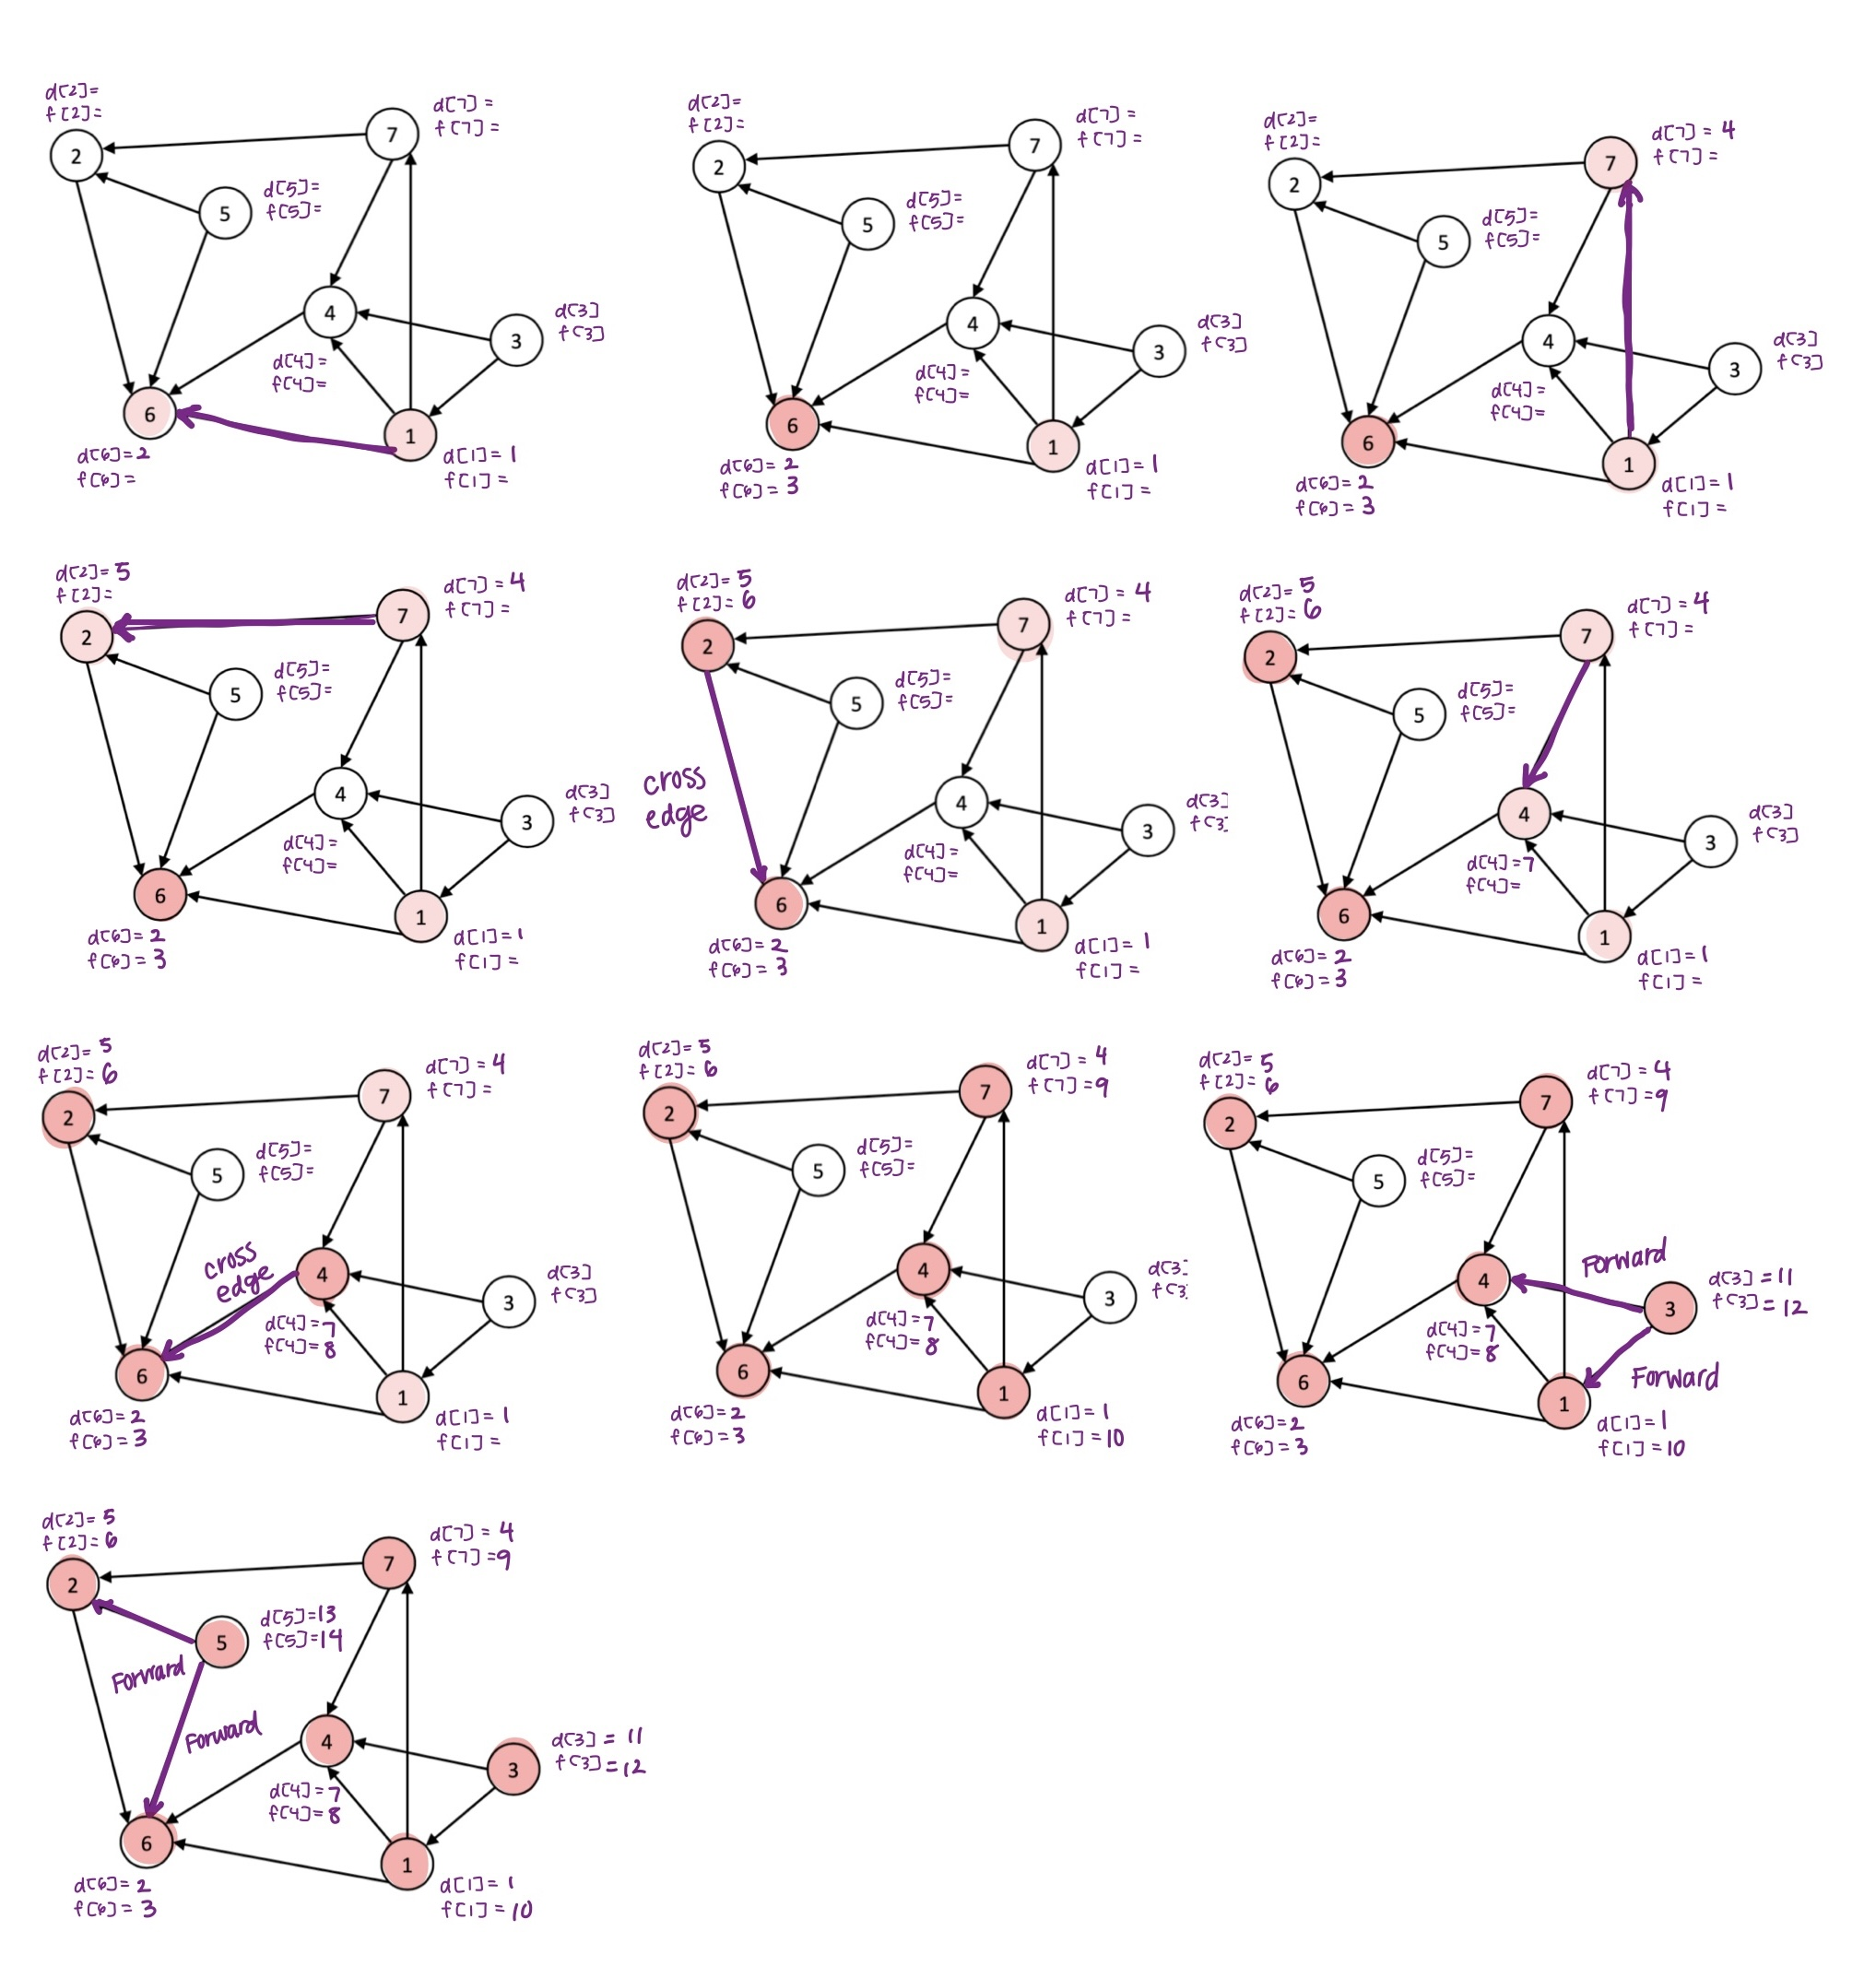
\includegraphics[width=0.3\textwidth]{Q1a.1.JPG}
        \caption{DFS Process}
        \label{f:Q1a.1}
\end{figure}

\begin{figure}[ht!]
        \centering
        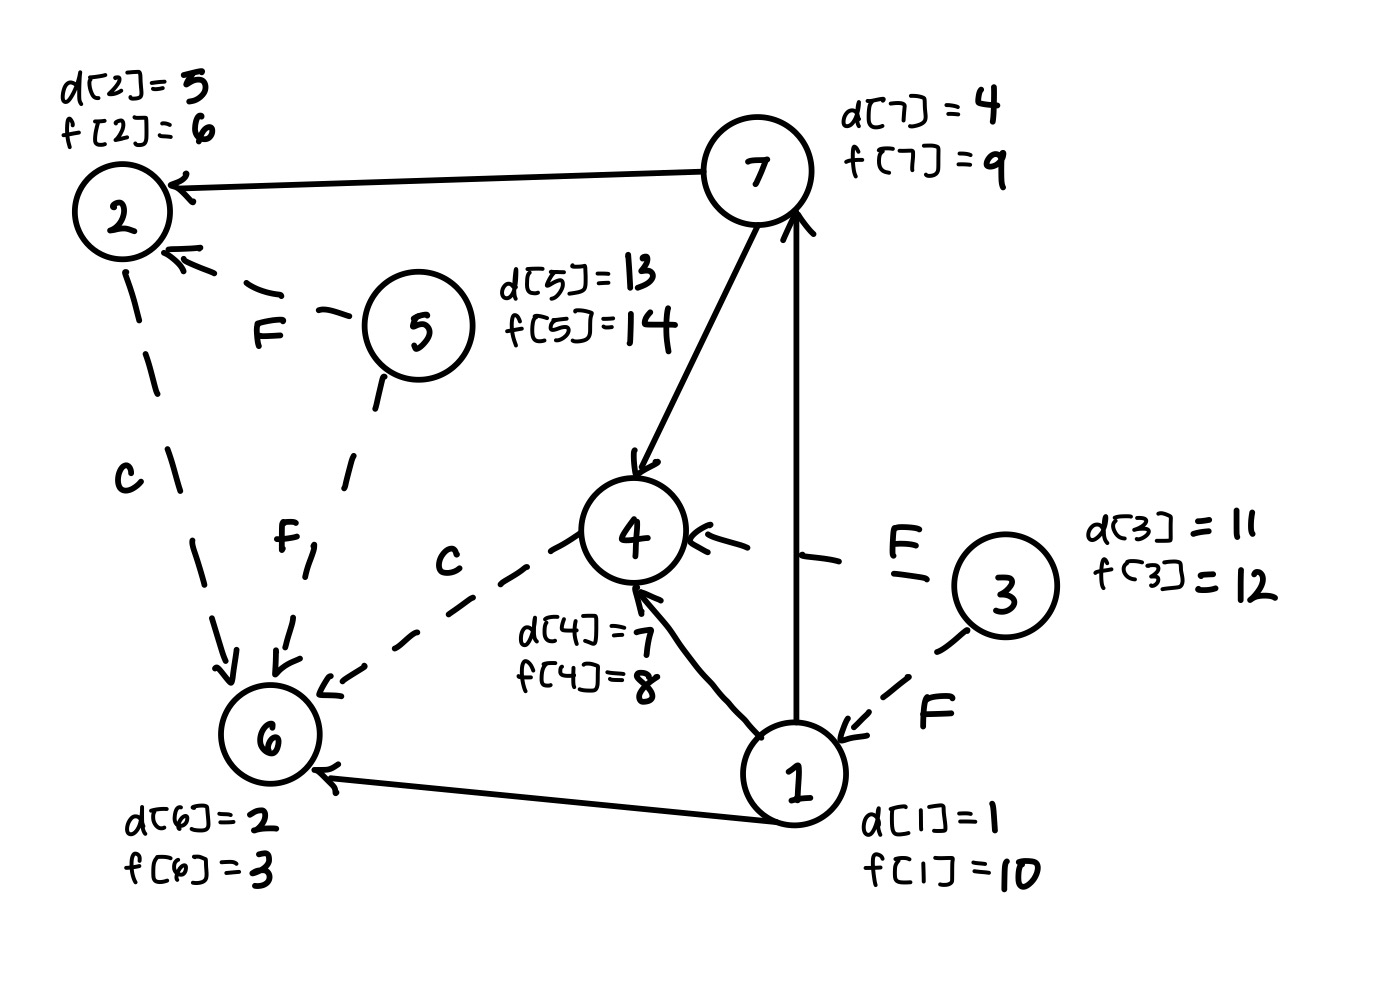
\includegraphics[width=0.3\textwidth]{Q1a.2.JPG}
        \caption{DFS forest starting at node 1.}
        \label{f:Q1a.2}
\end{figure}

\subsection*{Part (b)}
From the textbook, Lemma 22.11 says that a directed graph is acyclic if and only if a DFS yields no back edges. We also know from tutorial that G is acyclic if and only if an ordering is possible.\\
From part (a), there are no back edges in this DFS, and therefore the directed graph is acyclic. Therefore, we can conclude that an ordering is possible

\subsection*{Part (c)}
To obtain the list, we use Topological-Sort(G), which creates a linked list based on the finish times from greatest to least. Therefore, our order would be 5, 3, 1, 7. 4, 2, 6. Note that technically 3 could come before 5, but based on our DFS 3 is finished before 5.

\subsection*{Part (d)}
\begin{figure}[ht!]
        \centering
        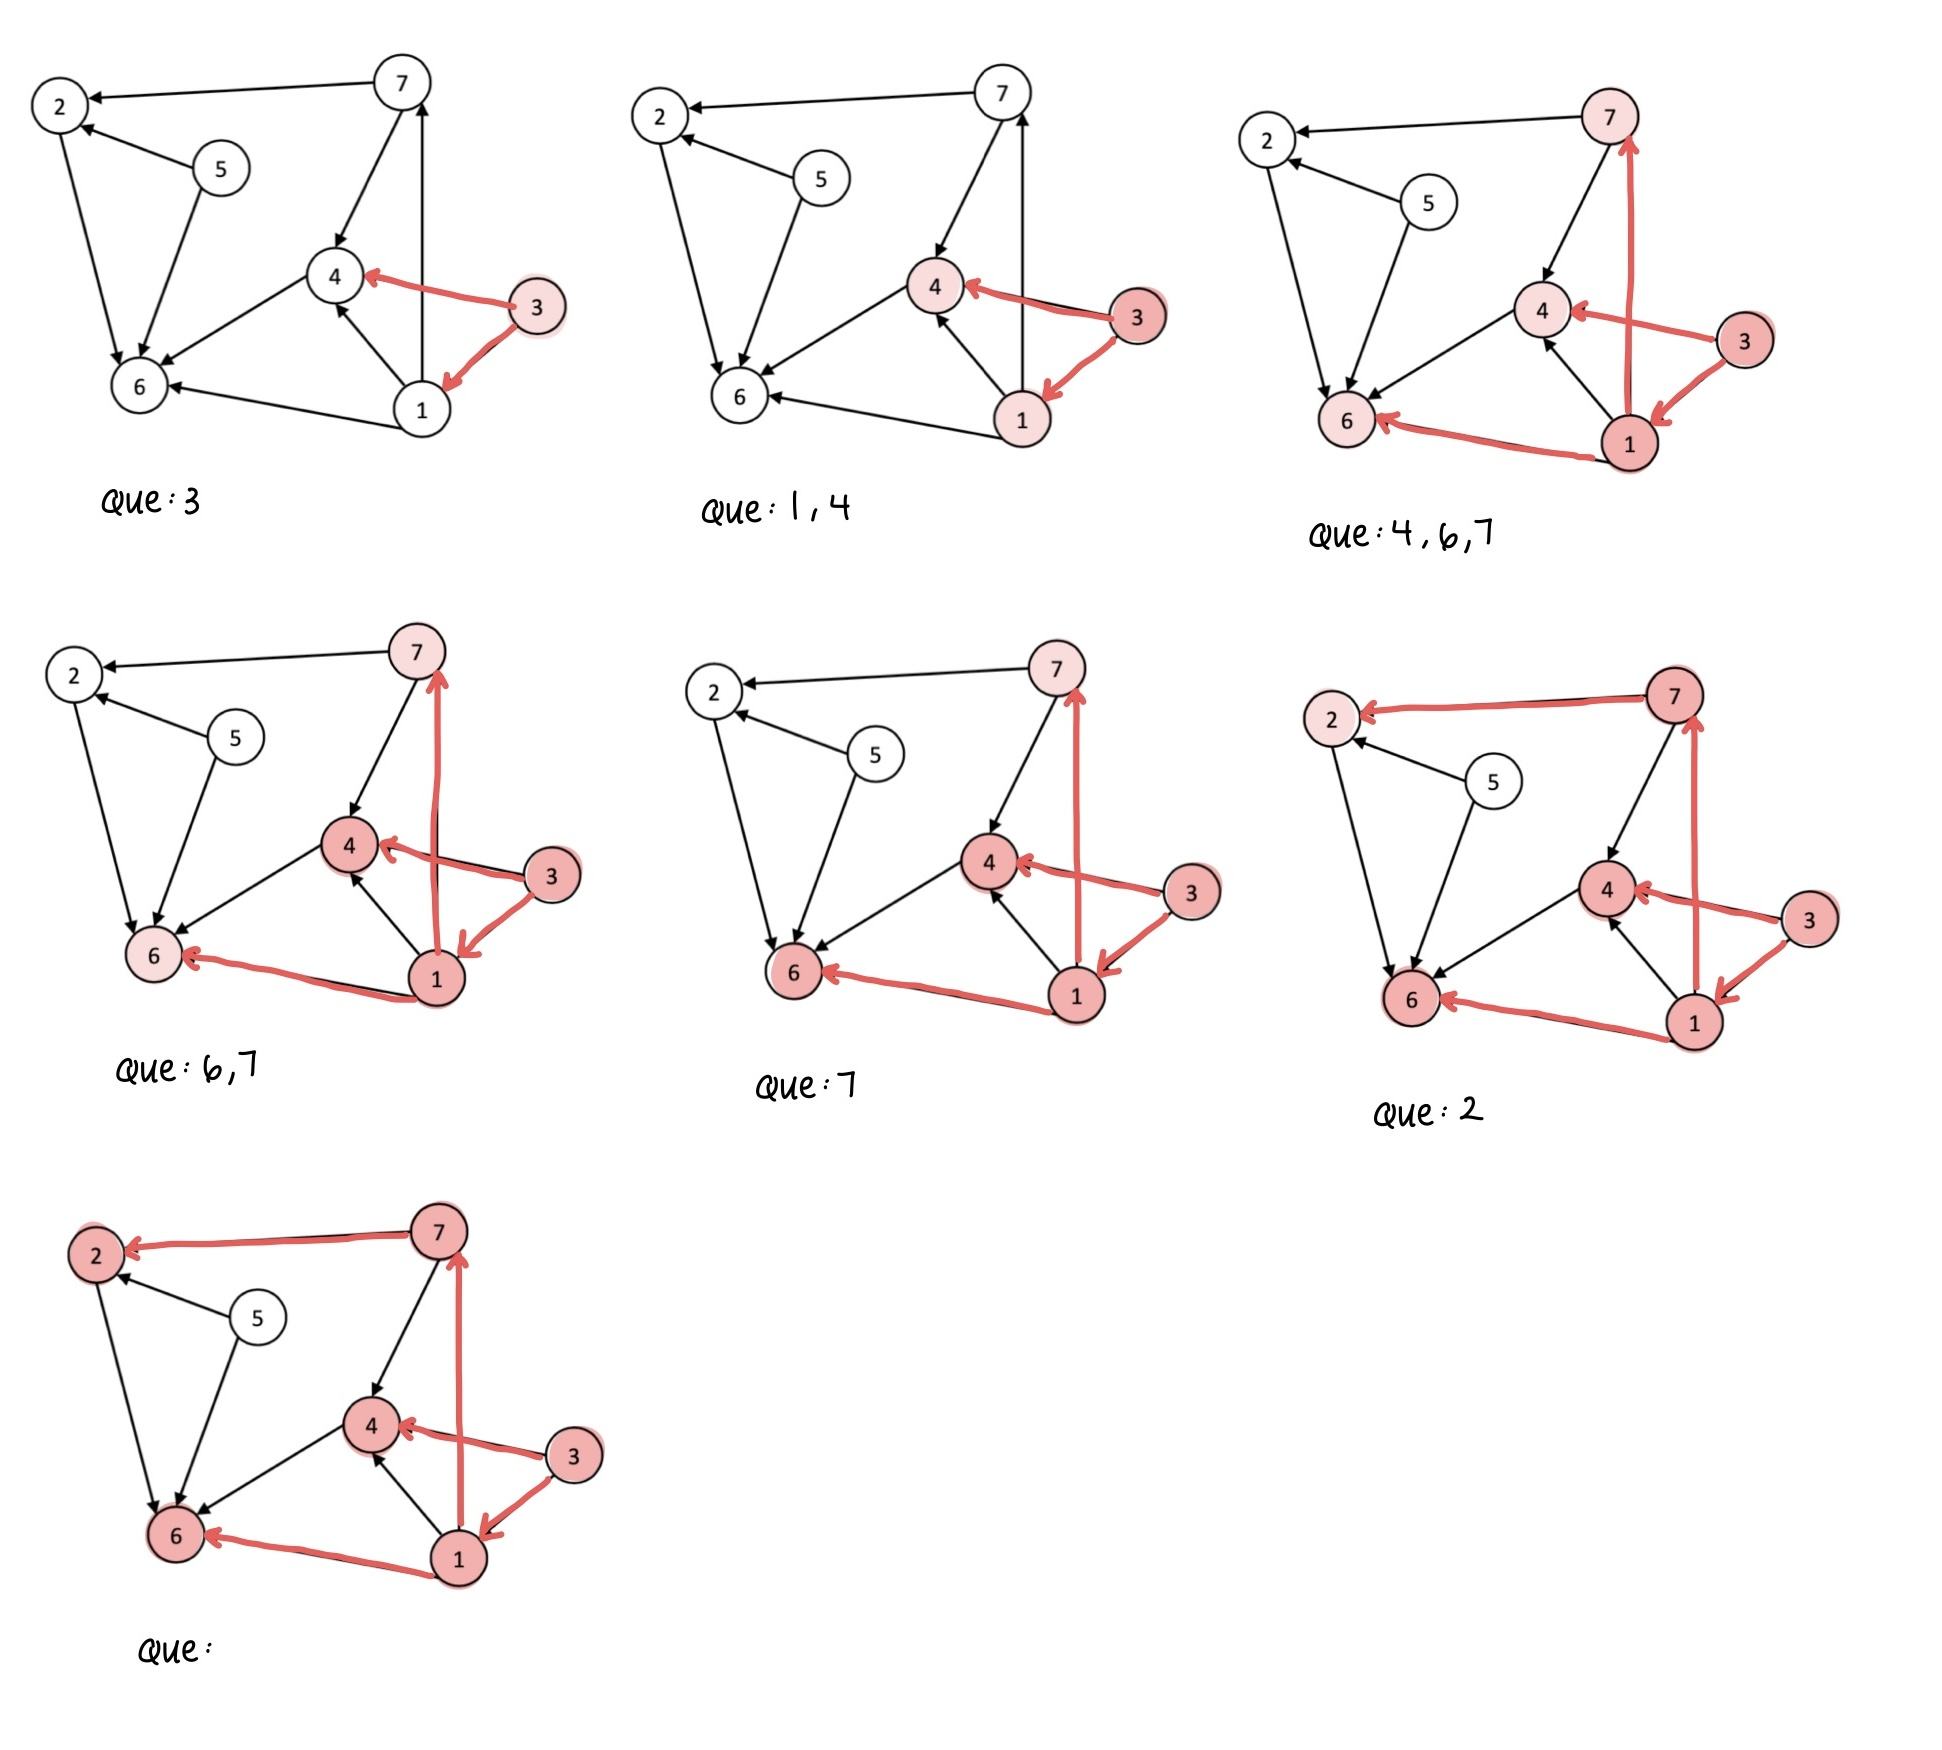
\includegraphics[width=0.3\textwidth]{Q1d.1.JPG}
        \caption{BFS Process}
        \label{f:Q1d.1}
\end{figure}

\begin{figure}[ht!]
        \centering
        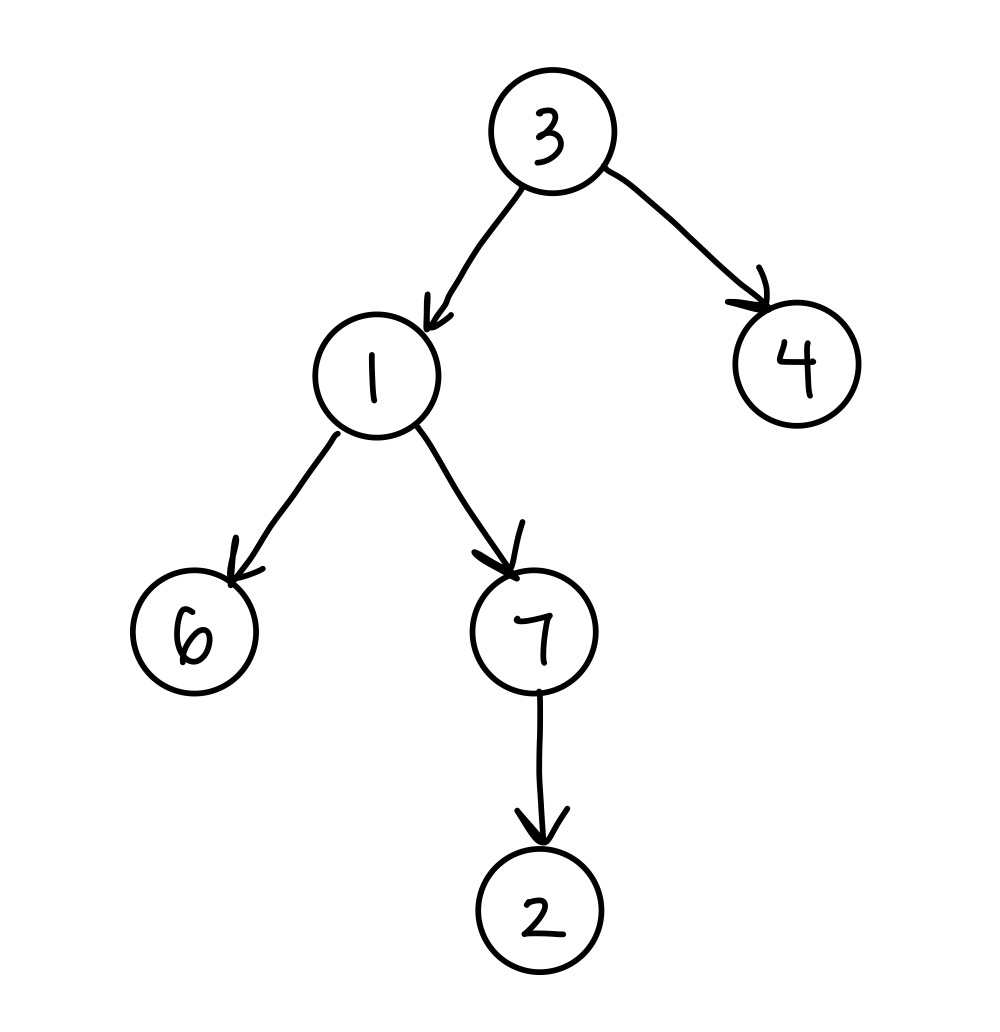
\includegraphics[width=0.3\textwidth]{Q1d.2.JPG}
        \caption{BFS tree starting at node 3.}
        \label{f:Q1d.2}
\end{figure}

\section*{Question 2 (written by Natalia, verified by Nena)}
\subsection*{Part (a)}
 By the negation of Lemma 22.11, a directed graph is acyclic if and only if a DFS yields no back edges. We also know from tutorial that G is acyclic if and only if an ordering is possible.\\
 \\
 Suppose the non-empty digraph is acyclic. We can then perform a topological sort to order the nodes. A topological sort is a linear ordering of all its vertices such that if G contains and edge (u,v), then u appears before v in the ordering. Suppose for the sake of contradiction that there are no sources. This means that the first node u in the linked list has to have an edge that points to it from node v. Therefore, v must appear before u. But this is a contradiction since node u is at the head of the list with no nodes before it. Therefore, there must be at least one source. 
\subsection*{Part (b)}

To prove that a digraph is acyclic if and only if the repeated application of the source-removal operation results in the empty graph, we proceed as follows: \\

\textbf{Proof (If Direction):} 

Assume that the repeated application of source removal leads to an empty graph. We will prove that the original graph must have been acyclic.

\begin{itemize}
    \item \textbf{Base Case:} Consider a graph with a single node. Removing this single source would immediately result in an empty graph. A single node without edges is trivially acyclic, satisfying the base case.
    \item \textbf{Inductive Step:} Assume that after \( n \) source removals, the graph was acyclic, meaning no cycles were present up to this point.
    
    \item Now consider adding an additional source node to this acyclic graph. Any additional source node would either have no edges or only edges pointing to nodes already in the graph, with no edges pointing back to itself or previous nodes (as there are no cycles by assumption).
    \item Thus, adding another source node does not create any cycles, and so the graph remains acyclic.
    \item By induction, if the repeated source-removal process leads to an empty graph, then the original graph must be acyclic.
\end{itemize}

\textbf{Proof (Only-If Direction):} 

Suppose the digraph is acyclic. 

\begin{itemize}
    \item Consider a non-empty digraph. Let us apply the source removal process repeatedly until it no longer can be applied.
    \begin{itemize}
        \item Case 1: the reason we can no longer apply the source removal is because the digraph is empty. Therefore, repeated application of source removal results in the empty graph.
        \item Case 2: the reason we can no longer apply the source removal is because the (non-empty) digraph has no more sources. Using the contrapositive of part (a), if there are no sources, then the non-empty digraph is NOT acyclic. However, this is a contradiction as we assumed that the digraph was acyclic (souce removals do not change this characteristic). Therefore, this case cannot happen.
    \end{itemize}
    \item  Note that a empty digraph (which is considered acyclic) holds because it is vacuously true (it is empty, therefore 0 source removals lead to an empty graph).
\end{itemize}


\subsection*{Part (c)}

To determine if a digraph is acyclic, we can use an algorithm based on the source-removal process from Part (b). This algorithm computes the in-degrees for all vertices, processes nodes with in-degree 0, and removes them from the graph. If all nodes can be processed in this manner, the graph is acyclic; otherwise, it contains a cycle. \\

\begin{algorithm}
\caption{IsAcyclic(G)}
\begin{algorithmic}[1]
    \State \( \text{inDegrees} \gets [0] \times |V| \) \Comment{Array to store the in-degree of each vertex}
    \State \( S \gets [] \) \Comment{Stack or queue to store vertices with in-degree 0 initially}

    \State \textbf{// Step 1: Initialize in-degrees for all nodes and populate initial sources}
    \For{each edge \( (u, v) \) in \( E \)}
        \State \( \text{inDegrees}[v] \gets \text{inDegrees}[v] + 1 \) \Comment{Increment in-degree of target node \( v \)}
    \EndFor
    \For{\( v \) in \( 0, 1, \dots, |V|-1 \)}
        \If{\( \text{inDegrees}[v] = 0 \)}
            \State \text{Append}(v, S) \Comment{Add \( v \) to \( S \) if it has in-degree 0}
        \EndIf
    \EndFor

    \State \textbf{// Step 2: Process vertices in \( S \) until it is empty}
    \While{\( S \) is not empty}
        \State \( s \gets \text{Pop}(S) \) \Comment{Remove a vertex \( s \) directly from \( S \)}

        \For{each edge \( (s, v) \) in \( E \)}
            \State \( \text{inDegrees}[v] \gets \text{inDegrees}[v] - 1 \) \Comment{Decrease the in-degree of the target node \( v \)}

            \If{\( \text{inDegrees}[v] = 0 \)}
                \State \text{Append}(v, S) \Comment{Add to \( S \) if it now has in-degree 0}
            \EndIf
        \EndFor
    \EndWhile

    \State \textbf{// Step 3: Check if all vertices were processed}
    \If{all \( \text{inDegrees}[v] = 0 \) for all \( v \) in \( 0, 1, \dots, |V|-1 \)}
        \State \textbf{return} True \Comment{No cycles detected, the graph is acyclic}
    \Else
        \State \textbf{return} False \Comment{There was a cycle in the graph}
    \EndIf
\end{algorithmic}
\end{algorithm}

\textbf{Explanation:}
\begin{itemize}
    \item \textbf{Step 1} initializes the in-degrees for each node and populates \( S \) with all nodes that have in-degree 0.
    \item \textbf{Step 2} processes each source \( s \) in \( S \), removing it and reducing the in-degrees of its neighbors. Any neighbor that reaches an in-degree of 0 is added to \( S \).
    \item \textbf{Step 3} checks if all nodes have been processed (i.e., if all in-degrees are 0). If so, the graph is acyclic; otherwise, it contains a cycle.
\end{itemize}

\subsection*{Part (d)}

To justify that the algorithm runs in \( O(n + m) \) time, where \( n \) is the number of nodes and \( m \) is the number of edges in the input graph, we analyze each part of the algorithm:

\begin{itemize}
    \item \textbf{Line 1:} Initializing the \texttt{inDegrees} array with zeroes takes \( O(n) \) time, as it involves setting an initial value for each of the \( n \) nodes.

    \item \textbf{Line 2:} Initializing \( S \) takes constant time.
    
    \item \textbf{Lines 3-6:} For each edge \( (u, v) \) in the graph, we increment the in-degree of the target node \( v \). This operation takes \( O(m) \) time, where \( m \) is the number of edges, since we process each edge once.
    
    \item \textbf{Lines 7-11:} We loop through each node \( v \) to check its in-degree. If its in-degree is zero, we add it to \( S \). This step takes \( O(n) \) time, as it involves examining each node exactly once.
    
    \item \textbf{Lines 12-21:} The \texttt{while} loop iterates as long as \( S \) is not empty. Each iteration removes a node \( s \) from \( S \) and processes its outgoing edges.

    \begin{itemize}
        \item In the worst case, each node will be a source node at some point and will need to be popped from S, and hence the while loop will run at most \( n \) times. 
        \item Furthermore, over all the iterations of the while loop, each edge is processed exactly once since each edge (s,v) corresponds to exactly one source node (namely \( s \)), so this edge will only be processed in the iteration of the while loop corresponding to that node. 
        \item Therefore, lines 12-21 take \( O(n + m) \) time in the worst case.
    \end{itemize}
    
    \item \textbf{Lines 23-27:} Finally, we check if all in-degrees are zero to confirm if all nodes have been processed. This involves a single pass through the \texttt{inDegrees} array, taking \( O(n) \) time.
\end{itemize}

Adding up the time for each step:

\[
O(n) + O(m) + O(n) + O(n + m) + O(n) = O(n + m)
\]

Thus, the total time complexity of the algorithm is \( O(n + m) \), which is efficient for this problem since each node and edge is only processed once.

\section*{Question 3 (written by both, verified by both)}
\subsection*{Part (a)}
Graph G = (V, E) where: 
\begin{itemize}
    \item V: the set of vertices of G representing the bike pump stations
    \item E: set of edges of G representing the straight bikeway that goes directly between any two bike pump station
    \item Edge weights: The Euclidian distance that you have to ride between any two successive bike station
\end{itemize}

\subsection*{Part (b)}
\textbf{Proof:} Let \( G \) be an undirected weighted graph, and \( T \) be any MST of \( G \). Let \( s \) and \( t \) be two distinct nodes of \( G \), and let \( P \) be the \( s \to t \) path in \( T \) (the only such path from \( s \) to \( t \) in \( T \)). \\

We want to show that \( P \) is a path with the minimum maximum edge weight among all paths from \( s \) to \( t \) in \( G \): 
\[
\forall P' \in G, \quad \max \text{EdgeWeight}(P) \leq \max \text{EdgeWeight}(P').
\]

\textbf{Formal Proof:}
\begin{enumerate}
    \item Let \( T' \) be an arbitrary spanning tree (possibly another MST) of \( G \). By definition of an MST:
    \begin{equation}
    \sum_{e \in T} w(e) \leq \sum_{e \in T'} w(e). \tag{1}
    \end{equation}
    
    \item Let \( P' \) be any path \( s \to t \) in \( G \). The path \( P \) consists entirely of edges in \( T \), while \( P' \) may contain edges not in \( T \).

    \item For \( P' \), we argue as follows:
    \begin{itemize}
        \item Since \( T \) is a spanning tree, it contains no cycles. Adding any edge \( e \notin T \) to \( T \) creates a cycle.
        \item By the minimum spanning tree property, any cycle created by adding \( e \notin T \) will always have at least one edge in \( T \) whose weight is less than or equal to the weight of \( e \notin T \). Since T is a min spanning tree, replacing \( e \notin T \) with an edge in \( T \) cannot increase the total weight of the path.
        \item This implies that any \( s \to t \) path (such as \( P' \)) containing edges not in \( T \) cannot have a smaller total weight than \( P \), which uses only edges in \( T \).
    \end{itemize}
    Thus, we conclude:
    \begin{equation}
    \sum_{e \in P} w(e) \leq \sum_{e \in P'} w(e). \tag{2}
    \end{equation}
    
    \item Next, consider the maximum edge weight. The maximum edge weight of \( P \) is, by definition, the largest edge weight among the edges of \( P \). Similarly, the maximum edge weight of \( P' \) is the largest edge weight among the edges of \( P' \).

    \begin{itemize}
        \item If \( P = P' \), then clearly:
        \[
        \max \text{EdgeWeight}(P) = \max \text{EdgeWeight}(P').
        \]
        \item If \( P \neq P' \), then \( P' \) must include edges not in \( T \), meaning \( P' \) is not part of the MST. Because \( T \) minimizes the maximum edge weight globally, any additional edges in \( P' \) cannot reduce the maximum edge weight below that of \( P \). Hence:
        \[
        \max \text{EdgeWeight}(P) \leq \max \text{EdgeWeight}(P').
        \]
    \end{itemize}

\end{enumerate}

\textbf{Conclusion:} We have shown that \( \forall P' \in G, \max \text{EdgeWeight}(P) \leq \max \text{EdgeWeight}(P') \), so \( P \) is the path with the minimum maximum edge weight among all paths from \( s \) to \( t \) in \( G \). \(\square\)


\subsection*{Part (c)}

\begin{itemize}
\item To solve the bike riding problem, the algorithm constructs a minimum spanning tree (MST) incrementally, starting from the vertices of \(G\). It uses Kruskal's algorithm to make sure that the maximum Euclidian distance is at a minimum. The steps are as follows:

\item First, a min-heap is built from the edges of \(G\), where each edge is prioritized by its weight. Additionally, each vertex in \(G\) is initialized as its own singleton set using a disjoint-set data structure.

\item The algorithm maintains an initially empty set \(MST\_Edges\), which will store the edges of the MST as they are added. (These edges will ultimately comprise the path from \(s\) to \(t\) we are looking for).

\item It iteratively extracts the minimum-weight edge from the heap. If the set representatives of the endpoints \(u\) and \(v\) are not the same (i.e., they are not yet connected in the MST), the edge \((u,v)\) is added to \(MST\_Edges\), and the sets of these endpoints are merged.

\item Every iteration of the while loop, the algorithm checks whether the set representatives of \(s\) and \(t\) belong to the same set after an edge is added. If so, it terminates early, as the \(s \to t\) path in the partially constructed MST has been completed. This path minimizes the maximum edge weight between \(s\) and \(t\).
\end{itemize}


\begin{algorithm} [H]
\caption{MinMaxDistance(G, s, t)}
\begin{algorithmic}[1]
\State \textbf{Input:} \( G \): a Graph that follows the definition in part a, \( s \): the starting node, \( t \): the ending node
\State \textbf{Output:} 
\\
\State $BuildMinHeap(E)$
\For{\( i = 1 \) to \(n\)}
        \State MakeSet(i)
    \EndFor
\State $MST\_edges \gets Ø$
\While{$MST\_edges < n - 1$}
    \State (u, v) $\gets$ $extract\_min(E)$
    \State r $\gets$ find(u)
    \State s $\gets$ find(v)
    \If{r != s}
        \State Union(r, s)
        \State $MST\_edges \gets MST\_edges\ U\ \{(u,v)\}$
    \EndIf

    \State a $\gets$ find(s)
    \State b $\gets$ find(t)
    \If{a == b}
        \State break
    \EndIf
\EndWhile
\end{algorithmic}
\end{algorithm}
\subsection*{Part (d)}
\begin{itemize}
    \item Line 4: BuildMinHeap takes O(m) time, where m is the number of edges.
    \item Lines 5-7: This for loop makes n singletons, which each take O(1) time. Therefore, this takes O(n) times total.
    \item Line 8: Initializing the set MST$\_$edges takes constant time O(1).
    \item Line 10: extract$\_$min takes O(log(n)) time. We are doing at most m extract$\_$min on a min heap the size of m. Therefore, in the worst case this will be O(mlogn)
    \item Lines 11-18: We are doing at most n-1 unions and 4m finds. We are also adding (u,v) to the MST edges at most n-1 times. Therefore, the total time in the worst case is O(m log*n + n).
    \item Lines 19-21: In the worst case, s and t will not be in the same set until we create the whole MST. Therefore, in the worst case this will not be called to end the algorithm early. 
\end{itemize}
In the worst case, combining all the big O's we get O(m + n + mlogn + mlog*n + n). Also, in the worst case there are (n-1) * (n-1) edges if each vertext is connected to every other vertex, therefore is about $n^{2}$. Simplifying the big O above by taking the largest element, this would give us a runtime of O$(n^{2}logn)$.
\end{document}
